\documentclass[acmtoms]{acmsmall} 


\usepackage{amsmath}
\usepackage{amsfonts}
\usepackage{amssymb}
\usepackage{graphicx}
\usepackage{url} 
\usepackage{color}
\usepackage[ruled,vlined]{algorithm2e}
\usepackage{subfig}
\usepackage{mathrsfs}
\usepackage{bm}
        
%% Our definition
\def\K{\mathbb{K}}
\def\N{\mathbb{N}}
\def\Z{\mathbb{Z}}
\def\F{\mathbb{F}}
\def\M{\mathsf{M}}
\def\C{\mathsf{C}}
\def\I{\mathsf{M}_{{\rm int}}}
\def\R{\mathsf{R}}
\def\Q{\mathbb{Q}}
\def\A{\mathbb{A}}

\def\Mat{\mathcal{M}}

\DeclareBoldMathCommand{\bA}{A}
\DeclareBoldMathCommand{\bL}{\mathcal{L}}
\DeclareBoldMathCommand{\bB}{B}
\DeclareBoldMathCommand{\bu}{u}
\DeclareBoldMathCommand{\bv}{v}
\DeclareBoldMathCommand{\bw}{w}


%\def\bigO{{\ensuremath{\operatorname{O}}}} 
%\def\bigO{{\ensuremath{\mathcal{O}}}}
%\markboth{}{}

\newcommand{\todo}[1]{(\textbf{todo:} #1)}

%% TeXmacs macros
\newcommand{\tmop}[1]{\ensuremath{\operatorname{#1}}}
\newcommand{\assign}{:=} 
\newcommand{\rem}{\tmop{rem}}

%% \setlength{\parindent}{0pt}

\title{
Simultaneous conversions with the Residue Number System using linear algebra
}
            
\author{
Javad Doliskani \affil{University of Waterloo}
Pascal Giorgi \affil{LIRMM CNRS - University of Montpellier}
Romain Lebreton \affil{LIRMM CNRS - University of Montpellier}
Eric Schost \affil{University of Waterloo}
}
           
\begin{abstract}
  We present an algorithm for simultaneous conversion between a given
  set of integers and their Residue Number System representations
  based on linear algebra. We provide a highly optimized
  implementation of the algorithm that exploits the computational
  features of modern processors.  The main application of our
  algorithm is matrix multiplication over integers. Our speed-up of
  the conversions to and from the residue number system significantly
  improves the overall running time of matrix multiplication.
\end{abstract}
      
\category{G.4}{Mathematical Software}{Algorithm design and analysis} 
\category{F.2.1}{Analysis of Algorithms and Problem Complexity}{Numerical Algorithms and Problems}[computations in finite fields.]
\terms{Algorithms, Experimentation, Performance.}
\keywords{}
            
\begin{document}
            
% \begin{bottomstuff}
% \end{bottomstuff}
            
\maketitle

%////////////////////////////////////////////////


\section{Introduction}


There currently exist a variety of high-performance libraries for
linear algebra or polynomial transforms using floating point
arithmetic~\cite{Whaley2001,Goto2008,FFTW05,Pueschel:05}.
High-performance kernels for linear algebra or polynomial arithmetic
are also available in the context of computations over the integers or
finite fields, through libraries or systems such as
NTL~\cite{Shoup95}, FLINT~\cite{Hart2010},
FFLAS-FPACK~\cite{fflas-ffpack} or Magma~\cite{BoCaPl97}.  

In this paper, we are interested in the latter kind of computation, in
the context of multiple precision arithmetic: we work with matrices or
polynomials with coefficients that are multi-precision integers, or
lie in a finite ring $\Z/N\Z$, for some large $N$, and we are
interested in the multiplication of these matrices or
polynomials. There exist multiple applications to this fundamental
operation; we illustrate this in the last section of this paper with a
discussion of polynomial factorization.

To perform a matrix or polynomial multiplication in such a context,
several possibilities exist. A first approach consists in applying
known algorithms, such as Strassen's, Karatsuba's, \dots directly over
our coefficient ring, relying {\it in fine} on fast algorithms for
multiplication of multi-precision integers. Another large class of
algorithms relies on {\em modular techniques}, or {\em residue number
  systems}, computing the required result modulo many small primes
before recovering the output by Chinese Remaindering.  One should not
expect either of these approaches to be superior in all
circumstances. For instance, in extreme cases such as the product of
matrices of size $1$ or $2$ with large integer entries, the modular
approach highlighted above is most likely not competitive with a
direct implementation. On the other hand, for the product of larger
matrices or polynomials, residue number systems often perform better
than direct ones, and as such, they are used in libraries or systems
such as NTL, FFLAS-FFPACK, Magma, \dots

In this paper, we present new techniques for residue number systems
that are applicable in a wide range of situations. In many cases, the
bottlenecks in such techniques are the reduction of the inputs modulo
many small primes, and the reconstruction of the output from its
modular images by means of Chinese Remaindering; by contrast,
operations modulo the small primes are often quite efficient.

Algorithms of quasi-linear complexity have been known for long for
both modular reduction and Chinese Remaindering, but their practical
performance remains somewhat lagging. Our algorithm offers an
alternative to these techniques, for those cases where we have several
coefficients to convert; it relies on matrix multiplication to perform
these tasks, with matrices that are integer analogues of Vandermonde
matrices and their inverses. As a result, while its complexity is
inferior to that of asymptotically fast methods, our algorithm behaves
extremely well in practice, as it allows us to rely on
high-performance libraries for floating point matrix multiplication.

%////////////////////////////////////////////////
%////////////////////////////////////////////////
%////////////////////////////////////////////////

\section{Preamble on polynomial matrix multiplication}

We start by discussing two tangentially related questions, both
concerning the cost of some computations with polynomial matrices of
small degree.

Let us first make a general comment on our multiplication
algorithms. Suppose we want to evaluate a $R$-bilinear map $U \times V
\to W$, for some free $R$-modules $U,V,W$ with bases
$\bu=(u_1,\dots,u_r)$, $\bv=(v_1,\dots,v_s)$ and
$\bw=(w_1,\dots,w_t)$. To do so, we will naturally use a {\em bilinear
  algorithm}. Such an algorithm $\bL=({\cal L},{\cal L}',{\cal L}'')$
is given by three sequences of linear forms
\begin{itemize}
\item $\rho$ linear forms ${\cal L}=(L_1,\dots,L_\rho)$ in $U^*$;
\item $\rho$ linear forms ${\cal L}'=(L'_1,\dots,L'_\rho)$ in $V^*$;
\item $t$ linear forms ${\cal L''}=(L''_1,\dots,L''_t)$ defined over $R^{\rho}$,
\end{itemize}
such that $\phi(f,g)$ is obtained as $\sum_{1 \le i \le t} L''_i\big(
L_1 (f)L'_1(g),\dots,L_\rho (f)L'_\rho(g)\big ) w_i$ for all $f,g$ in
$U \times V$. The integer $\rho$ is called the {\em rank} of $\bL$.
We will not discuss in any detail bilinear algorithms for matrix
multiplication, but we will review some existing algorithms for
polynomial multiplication in low degree.

\medskip

We start with a straightforward problem: given two polynomial matrices
$\bA$ and $\bB$, with $\bA=[A_{i,j}]_{1 \le i \le m, 1 \le j \le n}$
and $\bB=[B_{j,k}]_{1 \le j \le n, 1 \le k \le p}$, compute the
product $\bA \bB$. We assume that all entries of $A$ and $B$ are in
$\Z[x]_\kappa$, which denotes the set of polynomials in $\Z[x]$ of
degree less than $\kappa$, for some fixed integer $\kappa$. We are
interested here in the case where $\kappa$ is a small constant: in the
application we have in mind, $\kappa$ will be at most $3$.

In the case $\kappa=1$, we are simply doing matrix multiplication over
$\Z$; by seeing the inputs as polynomials with matrix coefficients, we
now explain how to reduce this problem to linear algebra over $\Z$ for
any value of $\kappa$. We start from a bilinear algorithm $\bL=({\cal
  L},{\cal L}',{\cal L}'')$ for polynomial multiplication
$\Z[x]_\kappa \times \Z[x]_\kappa \to \Z[x]_{2\kappa-1}$. For small
values of $\kappa$, to compute the product of two such polynomials $A$
and $B$, we will rely on the following choices:
\begin{itemize}
\item For $\kappa=2$, with $A=a_0+a_1 x$ and $B=b_0+b_1 x$, the
  smallest possible rank is $\rho=2$, using for instance Karatsuba's
  algorithm.  In this case, we can take ${\cal L}=(a_0, a_1,
  a_0+a_1)$, ${\cal L}'=(b_0, b_1, b_0+b_1)$ and ${\cal L}''=(c_0,
  c_1-c_0-c_2, c_2)$. It is customary to explain this algorithm as an
  evaluation / interpolation scheme that multiplies $A$ and $B$ modulo
  $x$, $x-1$ and $x-\infty$.
\item For $\kappa=3$, with $A=a_0+a_1 x+a_2 x^2$ and $B=b_0+b_1 x+b_2
  x^2$, the smallest possible rank is $5$, but we will use an
  algorithm of rank $\rho=6$; it is given by the following linear forms:
  \begin{itemize}
  \item ${\cal L}=(a_0,a_1,a_2,a_0-a_2,a_0+a_1+a_2,a_0+a_1-a_2)$
  \item ${\cal L}'=(b_0,b_1,b_2,b_0-b_2,b_0+b_1+b_2,b_0+b_1-b_2)$
  \item ${\cal L}''=(c_0, -(c_0 + c_1 + c_2) + (c_4 + c_5)/2, (c_0 + c_1
    + c_2) - c_3, -(c_0 + c_2) + c_3 + (c_4 -c_5)/2, c_2)$.
  \end{itemize}
  It corresponds to multiplying $A$ and $B$ modulo $x$, $x-1$, $x^2+1$,
  and $x-\infty$.
\end{itemize}
Once $\bL$ is chosen, to compute the matrix product $\bA\bB$, we apply
${\cal L}$ to all entries of $\bA$, ${\cal L}'$ to all entries of
$\bB$, and perform $\rho$ matrix multiplications between the
corresponding scalar matrices (where $\rho$ is the rank of
$\bL$). Finally, we recover $\bA \bB$ by applying ${\cal L}''$ to all
the scalar matrices we obtained in the previous step.  

\medskip

For our second problem, consider a family of polynomials
$\bB=(B_1,\dots,B_s)$ in $\Z[x]_n$, all with degree less than $n$,
together with $r$ families of polynomials $\bA_1,\dots,\bA_r$, with
$\bA_i=(A_{i,1},\dots,A_{i,s})$, all polynomials $A_{i,j}$ being in
$\Z[x]_\kappa$. As before, we assume that $\kappa$ is a small constant
(typically, we may have $\kappa \in \{1,2,3\}$). Our goal is to
compute the products
$$C_i = \bA_i \cdot \bB = \sum_{j=1}^s A_{i,j} B_j,\quad 1 \le i \le
r.$$ We now explain how to reduce
this problem to matrix multiplication over $\Z$.

The basic idea is well-known: our problem can be seen as matrix
product in sizes $(r \times s)$ and $(s \times 1)$, with entries in
respectively $\Z[x]_\kappa$ and $\Z[x]_n$. Assuming for simplicity
that $\kappa$ divides $n$, we can split the right-hand side into a
matrix of size $(s \times n/\kappa)$, with entries in $\Z[x]_\kappa$.
After doing the corresponding $(r \times s)$ by $(s \times n/\kappa)$
product, the recombination of the entries to recover the output of
our original problem takes linear time. 

For $\kappa=1$, we are simply multiplying integer matrices of
respective sizes $(r,s)$ and $(s,n)$. In general, since we are
multiplying polynomial matrices with entries in $\Z[x]_\kappa$, we can
apply the algorithm given previously. After choosing a bilinear
algorithm $\bL$ of rank $\rho$ for
multiplication $\Z[x]_\kappa \times \Z[x]_\kappa
\to\Z[x]_{2\kappa-1}$, the bulk of the computation is 
$\rho$ matrix products in sizes $(r, s)$ by $(s, n/\kappa)$.
\todo{Unify notation for the size of matrices}

%////////////////////////////////////////////////
%////////////////////////////////////////////////
%////////////////////////////////////////////////

\section{Conversions to and from Residue Number Systems}

%////////////////////////////////////////////////

\subsection{Definitions}

Three quantities, $\beta$, $\gamma$ and $\delta$ will be used throughout.
\begin{itemize}
\item The default representation of positive integers will use a
  positional number system for a fixed radix $2^\beta$: any positive
  integer $a \in \N$ can be uniquely written as $a = \sum_{i=0}^{n-1}
  a_i2^{\beta i}$ for some $a_i$'s in $\{0,\dots,2^\beta-1\}$ and with
  $a_{n-1} \ne 0$; a typical choice is $\beta=64$. 

\item Let $m_1, m_2, \dots, m_s$ be pairwise coprime positive
  integers, and let $M = m_1 m_2 \cdots m_s$. Then, any integer $a\in
  [0,\hdots,M-1]$ is uniquely determined by its residues $( [a]_1,
  [a]_2, \dots, [a]_s)$, with $[a]_i = a \bmod m_i$.  We assume that
  the moduli $m_i$ defining this residue number system satisfy $m_i
  < 2^\gamma$ for all $i$; possible values for $\gamma$ are
  $\gamma=16$, $20$, or even $60$. 

\item We will have to multiply matrices, which will be done using BLAS
  matrix multiplication; this imposes restrictions on the size of the
  operands. Explicitly, we will let $\delta$ be such that matrix
  multiplication in any size is feasible for integer matrices with
  entries in $\{0,\dots,2^\delta-1\}$. Possible value for
  $\delta$ are $16$ or $20$. 
  \todo{the size of the product shoul be bounded. Will be fixed later.}
  
  For simplicity of notation, we will assume that $\delta$ divides $\gamma$,
  and we let $\kappa=\gamma/\delta$.
\end{itemize}
We assume that any positive (?) integer $a$ written in basis $2^x$, for
$x$ in $\{\alpha,\beta,\gamma\}$, can be written in basis $2^y$,
for any $y$ in $\{\alpha,\beta,\gamma\}$, in linear time $O(\log(a))$.

In order to benefit from the RNS representation, one needs to be able
to convert back and forth between the positional and residual number
systems. In the following two subsections, we discuss approaches for
converting integers from the classic positional system to the residue
number system, and conversely, using linear algebra.

%////////////////////////////////////////////////

\subsection{Conversion to RNS}

We start with the conversion of integers in their positional
representation to their residue number system representation.  Our
input is a sequence of positive integers $a_1,\dots,a_r$, with $a_i <
2^L$ for all $i$, together with moduli $m_1,\dots,m_s$ as above, all
$m_j$'s satisfying $m_j < 2^\gamma$. Our goal is to compute $a_i \bmod
m_j$, for all $i,j$.

Our first step is to write all inputs in radix $2^\delta$. Precisely,
we will write $a_i = A_i(2^\delta,2^\gamma)$, for some polynomials
$A_i$ in $\Z[x,y]$ of degree less than $\kappa$ in $x$ and $L/\gamma$
in $y$ \todo{rounding?}, and with non-negative coefficients less than
$2^\delta$. Explicitly, we have $A_i =\sum_{0 \le k < L/\gamma}
A_{i,k}(x) y^k$.

On the other hand, for any modulus $m_j$, and any positive integer
$k$, let us write the expansion of $2^{\gamma k} \bmod m_j$ 
in radix $2^\delta$ as
\begin{align*}
2^{\gamma k} \bmod m_j &=b_{j,k,0}+b_{j,k,1}2^{\delta} + \cdots +b_{j,k,\kappa-1}2^{(\kappa-1)\delta} \\  
&=B_{j,k}(2^\delta),
\end{align*}
where $B_{j,k}$ is the polynomial $B_{j,k}=b_{j,k,0}+b_{j,k,1}x +
\cdots +b_{j,k,\kappa-1}x^{\kappa-1} \in \Z[x]$.  As a result, we
obtain the equality
$$a_i \bmod m_j = C_{i,j}(2^\delta) \bmod m_j,$$ where $C_{i,j}$ is
the polynomial $\sum_{0 \le k < L/\gamma} A_{i,k} B_{j,k}$.  Hence, we
first compute the polynomials $C_{i,j}$, as deducing $a_i \bmod m_j$
is then straightforward using the above expression.  We are thus
reduced to performing a matrix product in size $(r \times L/\gamma)$
by $(L/\gamma,s)$, with polynomial entries of degree less than
$\kappa$ and coefficients in $\{0,\dots,2^\gamma-1\}$. To illustrate
the construction, we discuss two useful cases:
\begin{itemize}
\item Suppose that all moduli $m_j$ are bounded by $2^{16}$; in that 
  case, we have $\gamma=\delta=16$ and $\kappa=1$. In other words,
  we are doing scalar matrix multiplication, and the right-hand matrix
  $\bB=[B_{i,j}]$ is an analogue of a Vandermonde matrix, with 
  entries that are simply the values $2^{16 k} \bmod m_j$.
\item Consider now the case where all moduli $m_j$ are bounded by
  $2^{60}$.  In that case, we take $\delta=20$ and thus $\kappa=3$.
  We are thus left to perform a matrix product with entries that are
  polynomials of degree at most $2$ and with coefficients that are at
  msot $2^{20}$.
\end{itemize}

%////////////////////////////////////////////////

\subsection{Conversion from RNS}

We next consider the converse operation, Chinese Remaindering.
Let $a$ be an integer given by its RNS representation $([a]_1, \dots,
[a]_s)$ with base $(m_1,\dots,m_s)$. The unique integer $a$ in
$\{0,\dots,M-1\}$ satisfying all congruences $[a]_i = a \bmod m_i$ 
is
\begin{equation}\label{eq:cra}
a = \sum_{i=1}^s \left( [a]_i u_i \bmod m_i\right) \lambda_i  \bmod M,
\end{equation}
where we write $\lambda_i = M/m_i$ and $u_i = 1/\lambda_i \bmod m_i$ for all
$i$. 

In what follows, we are interested in the reconstruction of {\em
  several} such $a$s, say $a_1,\dots,a_r$, from their respective
residues $([a_i]_1, \dots, [a_i]_s)$, for $i=1,\dots,r$.  In this
case, $M$, all $\lambda_i$s and $u_i$s can be precomputed once and for
all.  We perform an operation we will call \textit{simultaneous
  pseudo-reconstructions} as follows.  For $i=1,\dots,r$ and
$j=1,\dots,s$, let $v_{i,j} = [a_i]_{j} u_j \bmod m_j$ and define
\[
b_i = \sum_{j=1}^s v_{i,j} \lambda_j,
\]
so that $a_i = b_i \bmod M$, and $b_i < M s$; we call $b_i$ the {\em
  pseudo-reconstruction} of $([a_i]_1,\dots,[a_i]_s)$ modulo $m_1,
\ldots, m_s$ \todo{better to integrate $u_j$ into $M_j$}. Once we know
$b_i$, we deduce $a$ itself using one Euclidean division. \todo{say a
  bit more}.

As we did for the previous conversion, we will use matrix
multiplication to compute all $b_i$s, which means that all operands
must be written in base $2^\delta$, as
\[v_{i,j} = \sum_{k=0}^{\kappa-1} v_{i,j,k}2^{k \delta}\
\quad\text{and}\quad
\lambda_j = \sum_{\ell = 0}^{L/\delta-1} \lambda_{j,\ell}2^{\ell \delta}.\]
These two integers can then be identified with the values of 
\[V_{i,j} = \sum_{k=0}^{\kappa-1} v_{i,j,k}x^{k}
\quad\text{and}\quad
\Lambda_j = \sum_{\ell = 0}^{L/\delta-1} \lambda_{j,\ell}x^{\ell}\]
at $2^\delta$. Hence, we will compute the polynomials 
$B_1,\dots,B_r \in \Z[x]$ defined as 
\[B_i = \sum_{j=1}^s V_{i,j} \Lambda_j\]
before deducing their value at $2^\delta$. 

\section{Application}

The following graph gives timings for the multiplication of
polynomials with 12000-bit coefficients using either NTL, or a
modification of it based on the algorithm above. For such degree and
bit-size ranges, NTL uses an algorithm based on Chinese Remaindering,
reducing the input modulo several FFT primes of about 60 bits. We
replaced the built-in reduction (that uses standard algorithms based
on subproduct trees) by an implementation of the algorithms described above.

\begin{center}
  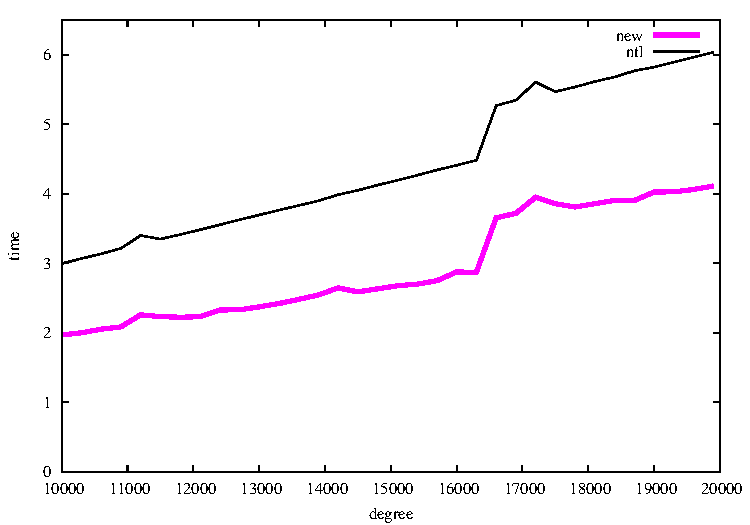
\includegraphics[width=11cm]{BENCH/bench12000.pdf}
\end{center}

\bibliographystyle{ACM-Reference-Format-Journals}
\bibliography{biblio}
\end{document}
  
